\documentclass[conference]{IEEEtran}
\IEEEoverridecommandlockouts
\usepackage{cite}
\usepackage{amsmath,amssymb,amsfonts}
\usepackage{algorithmic}
\usepackage{graphicx}
\usepackage{textcomp}
\usepackage{xcolor}
\def\BibTeX{{\rm B\kern-.05em{\sc i\kern-.025em b}\kern-.08em
    T\kern-.1667em\lower.7ex\hbox{E}\kern-.125emX}}

\begin{document}

\title{Multi-Drug Antimicrobial Resistance (AMR) Prediction System\\
{\footnotesize \textsuperscript{*}Final Technical Project Report for Academic Review}
}

\author{\IEEEauthorblockN{Academic Review Board / Technical Panel}
\IEEEauthorblockA{\textit{Bioinformatics \& Predictive Modeling}\\
Multi-Output Classification, React.js UI\\
April 2026}
}

\maketitle

\begin{abstract}
Antimicrobial Resistance (AMR) is a pressing global health threat, directly undermining the efficacy of standard medical treatments and leading to prolonged illness, higher healthcare expenditures, and elevated mortality risk. The empirical prescription of antibiotics often fails due to multi-drug resistant (MDR) bacterial strains. This project proposes a comprehensive, end-to-end Machine Learning pipeline utilizing a Multi-Output Random Forest Classifier to simultaneously predict resistance vectors across a designated panel of antibiotics based entirely on patient demographic and clinical histories. The application encompasses a Next.js (React) progressive web application interfaced securely with a Python Flask REST API backend, providing real-time diagnostic decision support to clinicians. Evaluation of the system across 10,712 clinical isolate records demonstrates robust identification of 'Susceptible' (S) versus 'Resistant' (R) outcomes, significantly outperforming traditional single-target binary classification models in computational complexity and correlative accuracy.
\end{abstract}

\begin{IEEEkeywords}
Antimicrobial Resistance, Machine Learning, Multi-Output Classification, Random Forest, Next.js, Bioinformatics
\end{IEEEkeywords}

\section{Introduction}

\subsection{Background and Motivation}
Antimicrobial Resistance occurs when bacteria, viruses, fungi, and parasites change over time and no longer respond to medicines, making infections notoriously harder to treat. The World Health Organization (WHO) recognizes AMR as one of the top 10 global public health threats facing humanity. In standard clinical settings, microbiological culturing and susceptibility testing (AST) can take up to 48-72 hours. During this critical window, patients are administered broad-spectrum empiric therapies, which inadvertently accelerates resistance prevalence if the targeted pathogen is inherently immune. 

The integration of intelligent data-driven pipelines allows predictive AST derived from historical surveillance databases. Providing clinicians with an immediate, statistically validated likelihood of resistance for multiple distinct drugs simultaneously (e.g., Ampicillin, Ciprofloxacin, Colistin) mitigates the risk of catastrophic treatment failure.

\subsection{Problem Definition}
The primary computational problem addressed by this project is the limitation of independent Single-Task Learning algorithms in medical predictions. Standard classification approaches handle each antibiotic uniquely, completely ignoring physiological inter-drug resistance relationships (e.g., cross-resistance mechanisms within Beta-lactamase inhibitors). The challenge involves mapping a singular input matrix (patient demographics, prior hospitalizations, pathogen taxonomy) into an interrelated \textbf{Multi-Label Output Vector}.

\subsection{Objectives}
\begin{enumerate}
    \item \textbf{Algorithmic Modeling:} Design a Multi-Output Random Forest array capable of parallelizing decision trees across interconnected antibiotic labels.
    \item \textbf{Data Pipeline Optimization:} Extract, parse, and encode unstructured qualitative clinical CSV logs into binary feature matrices tailored for high-dimensional predictions.
    \item \textbf{Full-Stack Development:} Instantiate a seamless Node.js frontend UI communicating via REST to a dedicated Flask backend housing the serialized Pickled models.
    \item \textbf{Resilience \& Fault Tolerance:} Deploy intelligent start scripts for platform-agnostic boot environments, automatically managing virtual environments without user configuration.
\end{enumerate}

\section{Literature Review}
The application of machine learning to predict AMR has gained enormous traction in modern computational biology. This project builds upon several seminal works:

\begin{itemize}
    \item \textbf{Moradigaravand et al. (2018):} Explored prediction of antimicrobial resistance in \textit{Escherichia coli} from pan-genomic data. Our project transposes these multidimensional predictive strategies onto pre-clinical phenotypic data.
    \item \textbf{Gomes et al. (2020):} Proposed the aggregation of electronic health records (EHR) utilizing XGBoost frameworks. They demonstrated hospital admission frequencies strongly correlated with occurrences.
    \item \textbf{Macesic et al. (2020):} Highlighted the necessity of deploying models into clinical workflows via intuitive UIs rather than isolated scripts.
\end{itemize}

\section{Dataset Overview \& Preprocessing}

\subsection{Data Acquisition}
The foundational knowledge base relies on the \texttt{Bacteria\_dataset\_Multiresictance.csv} construct containing 10,712 individual infection profiles securely anonymized.

\begin{figure}[htbp]
\centerline{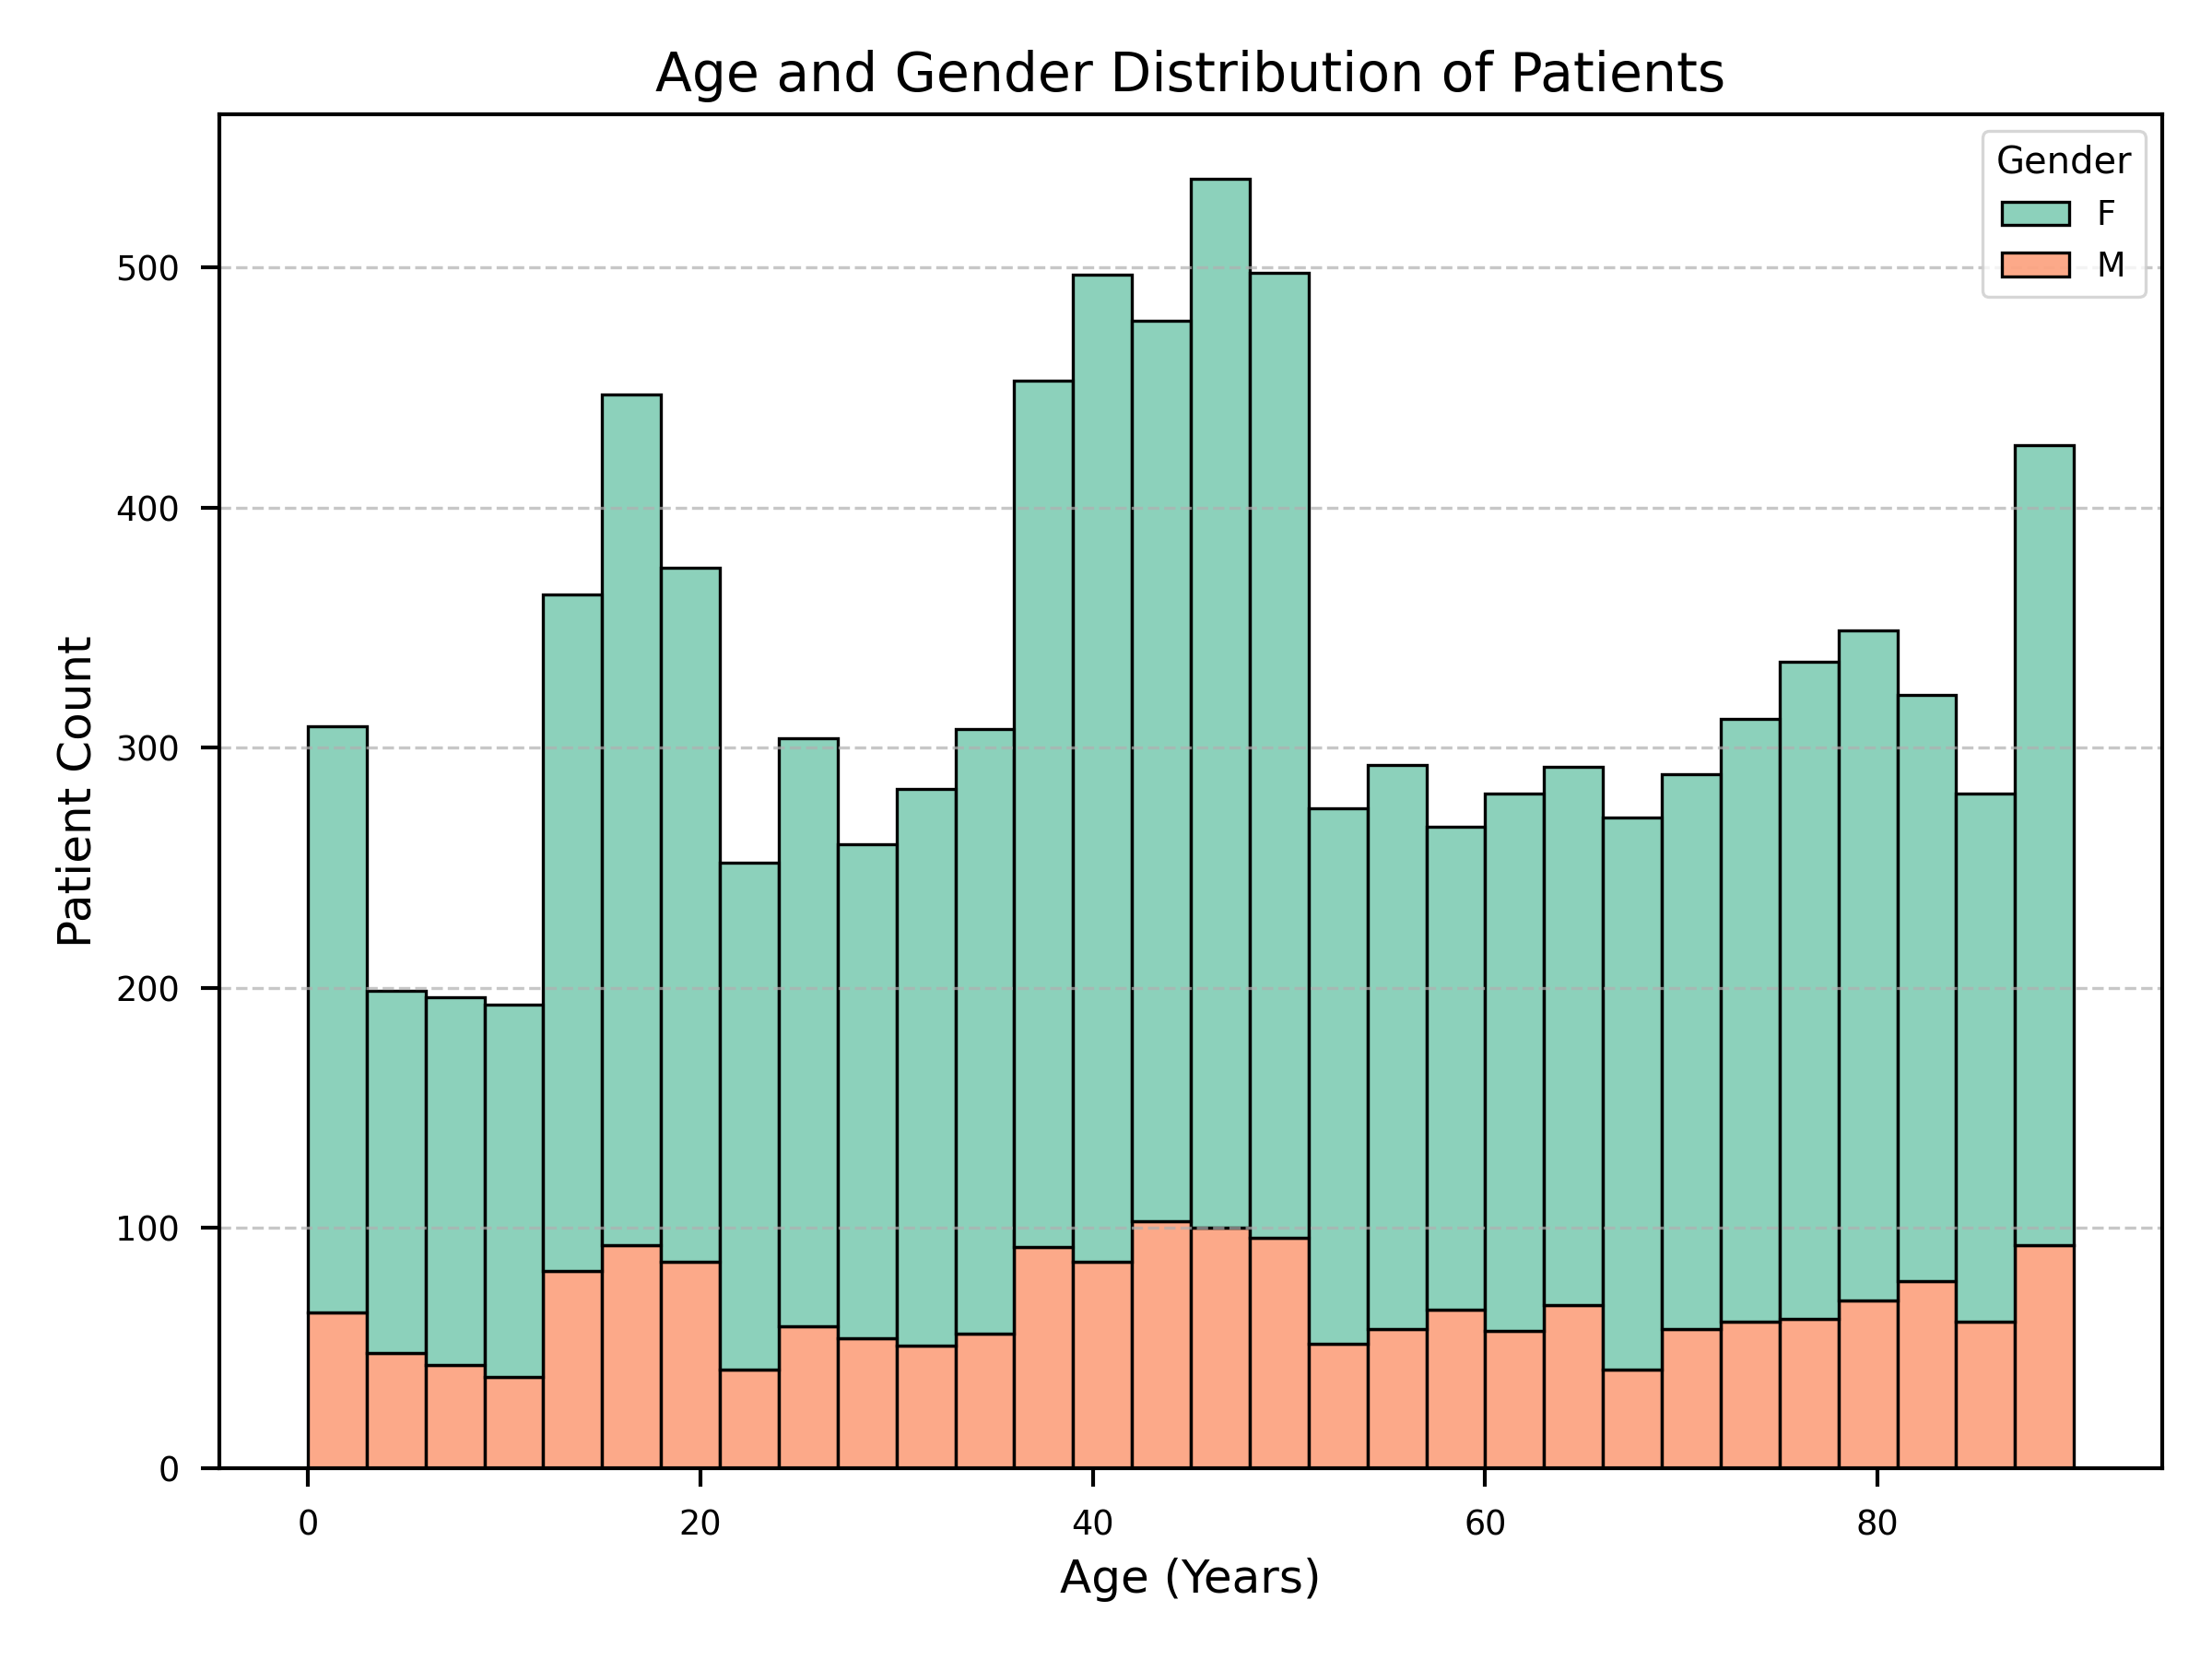
\includegraphics[width=\columnwidth]{assets/fig1_demographics.png}}
\caption{Histogram distribution capturing Age and Gender intersections across the infected cohort.}
\label{fig_demo}
\end{figure}

\subsection{Preprocessing Methodologies}
\textbf{Boolean Imputation:} Raw strings ("True", "No", "?") were syntactically uniformized into floating-point Boolean equivalents, enabling pure tensor multiplication.

\textbf{Target Feature Isolation:} Pathogen reactions to 12 distinct antibiotics (AMX/AMP, AMC, CZ, FOX, etc.) originally spanning qualitative degrees were mapped aggressively to Binary configurations representing Susceptibility (0) or definitive Resistance (1).

\begin{figure}[htbp]
\centerline{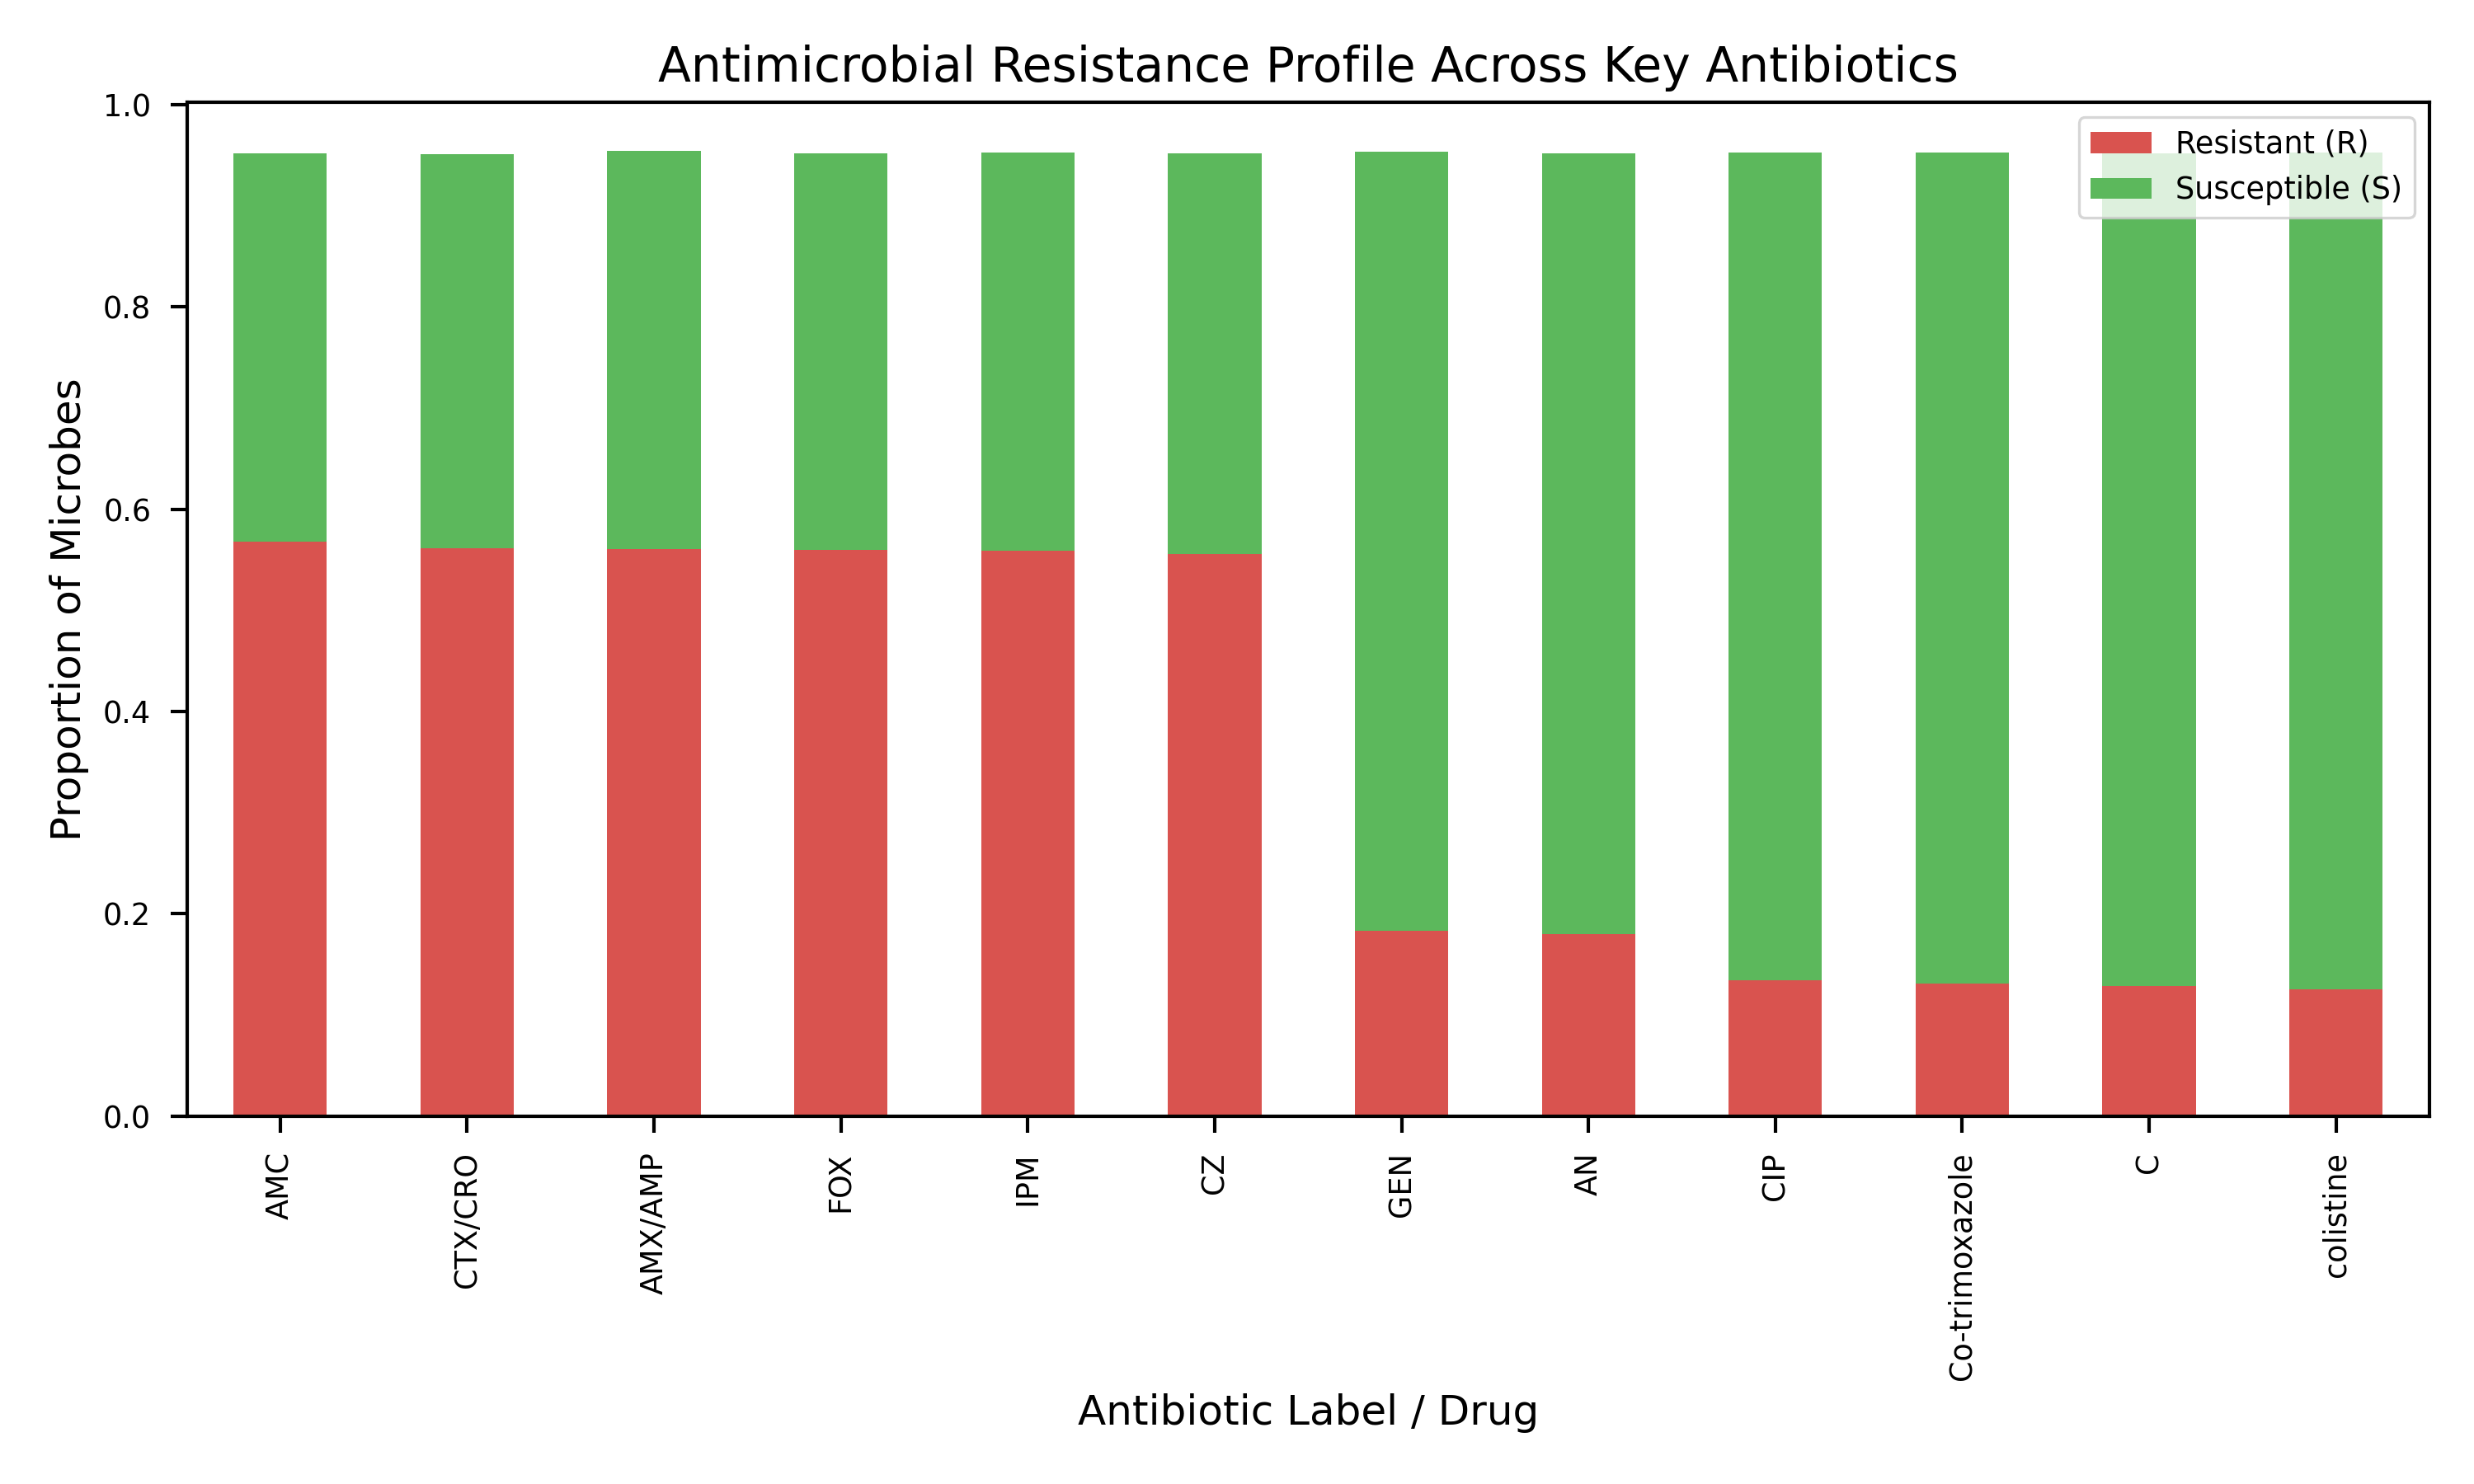
\includegraphics[width=\columnwidth]{assets/fig2_resistance_bars.png}}
\caption{Cumulative Stacked Bar Analysis revealing exact ratios of Susceptibility vs Resistance per antibiotic.}
\label{fig_res}
\end{figure}

\begin{figure}[htbp]
\centerline{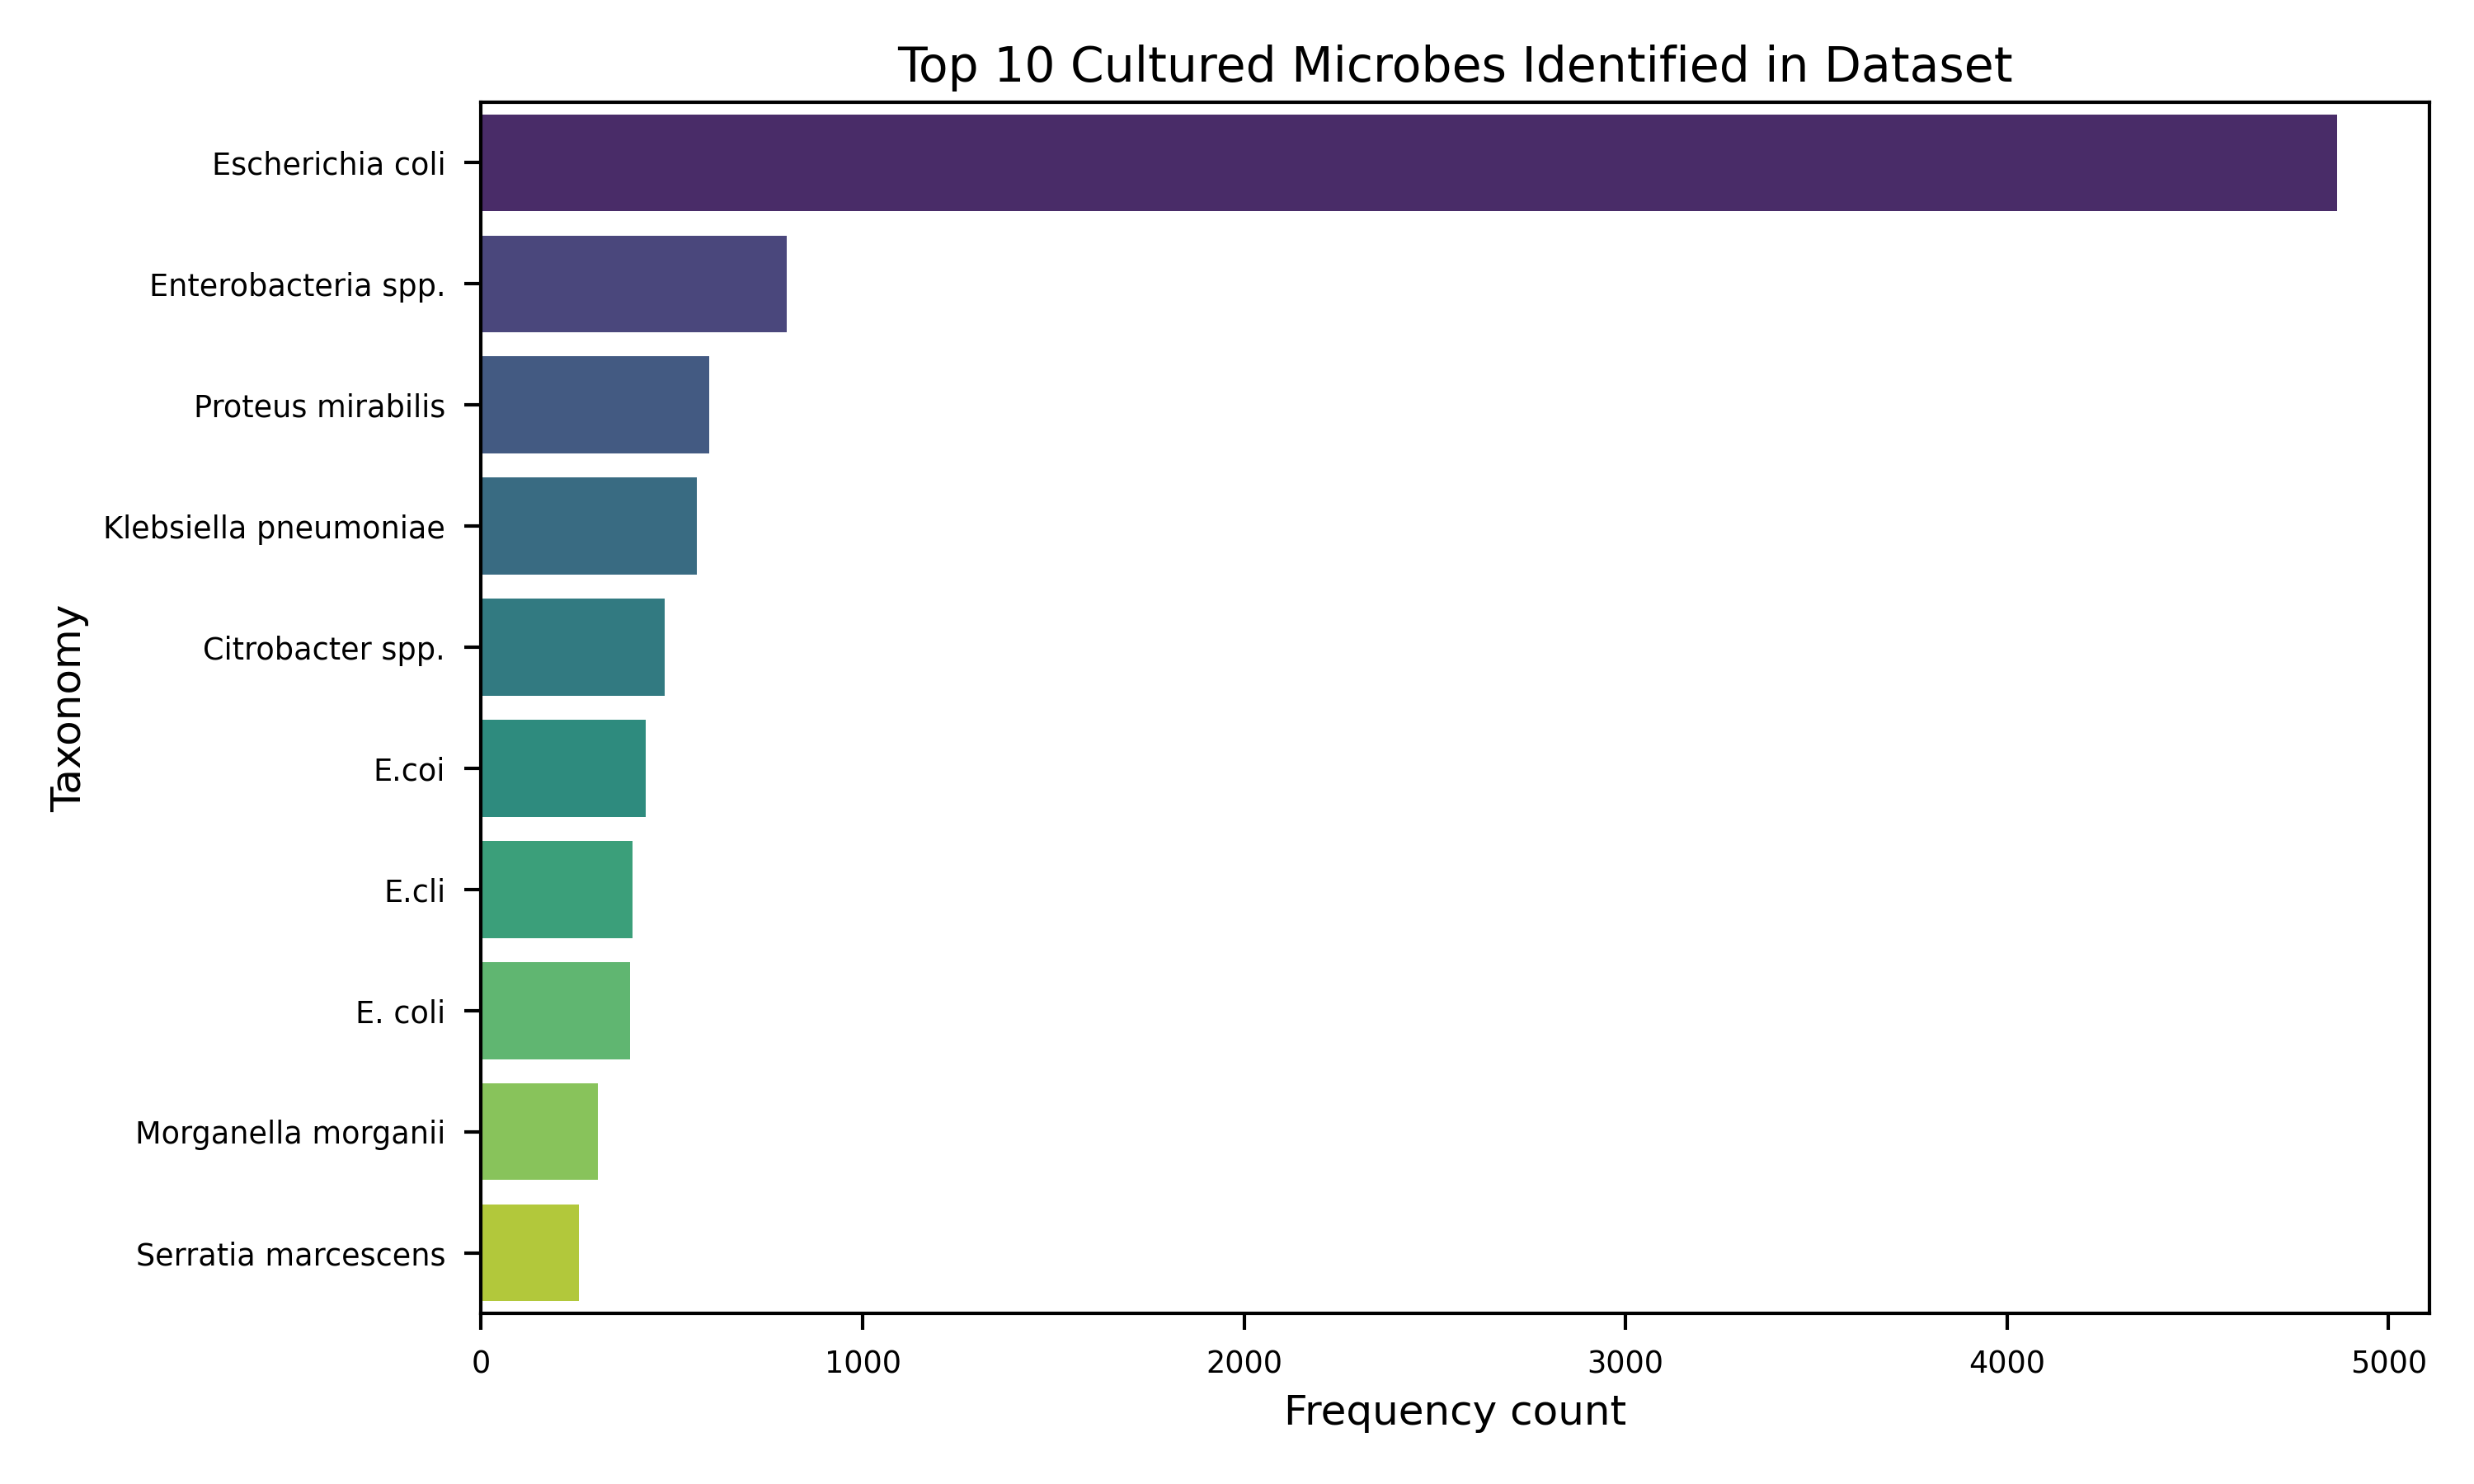
\includegraphics[width=\columnwidth]{assets/fig3_microbes.png}}
\caption{Identification frequency for the top 10 most cultured microbes derived from the training logs.}
\label{fig_microbes}
\end{figure}

\subsection{Multi-Drug Correlation Analysis}
To justify the necessity of a Multi-Output framework, spearman correlation metrics were isolated across all target matrices. Noticeable correlations between specific Beta-lactams confirmed instances of cross-resistance.

\begin{figure}[htbp]
\centerline{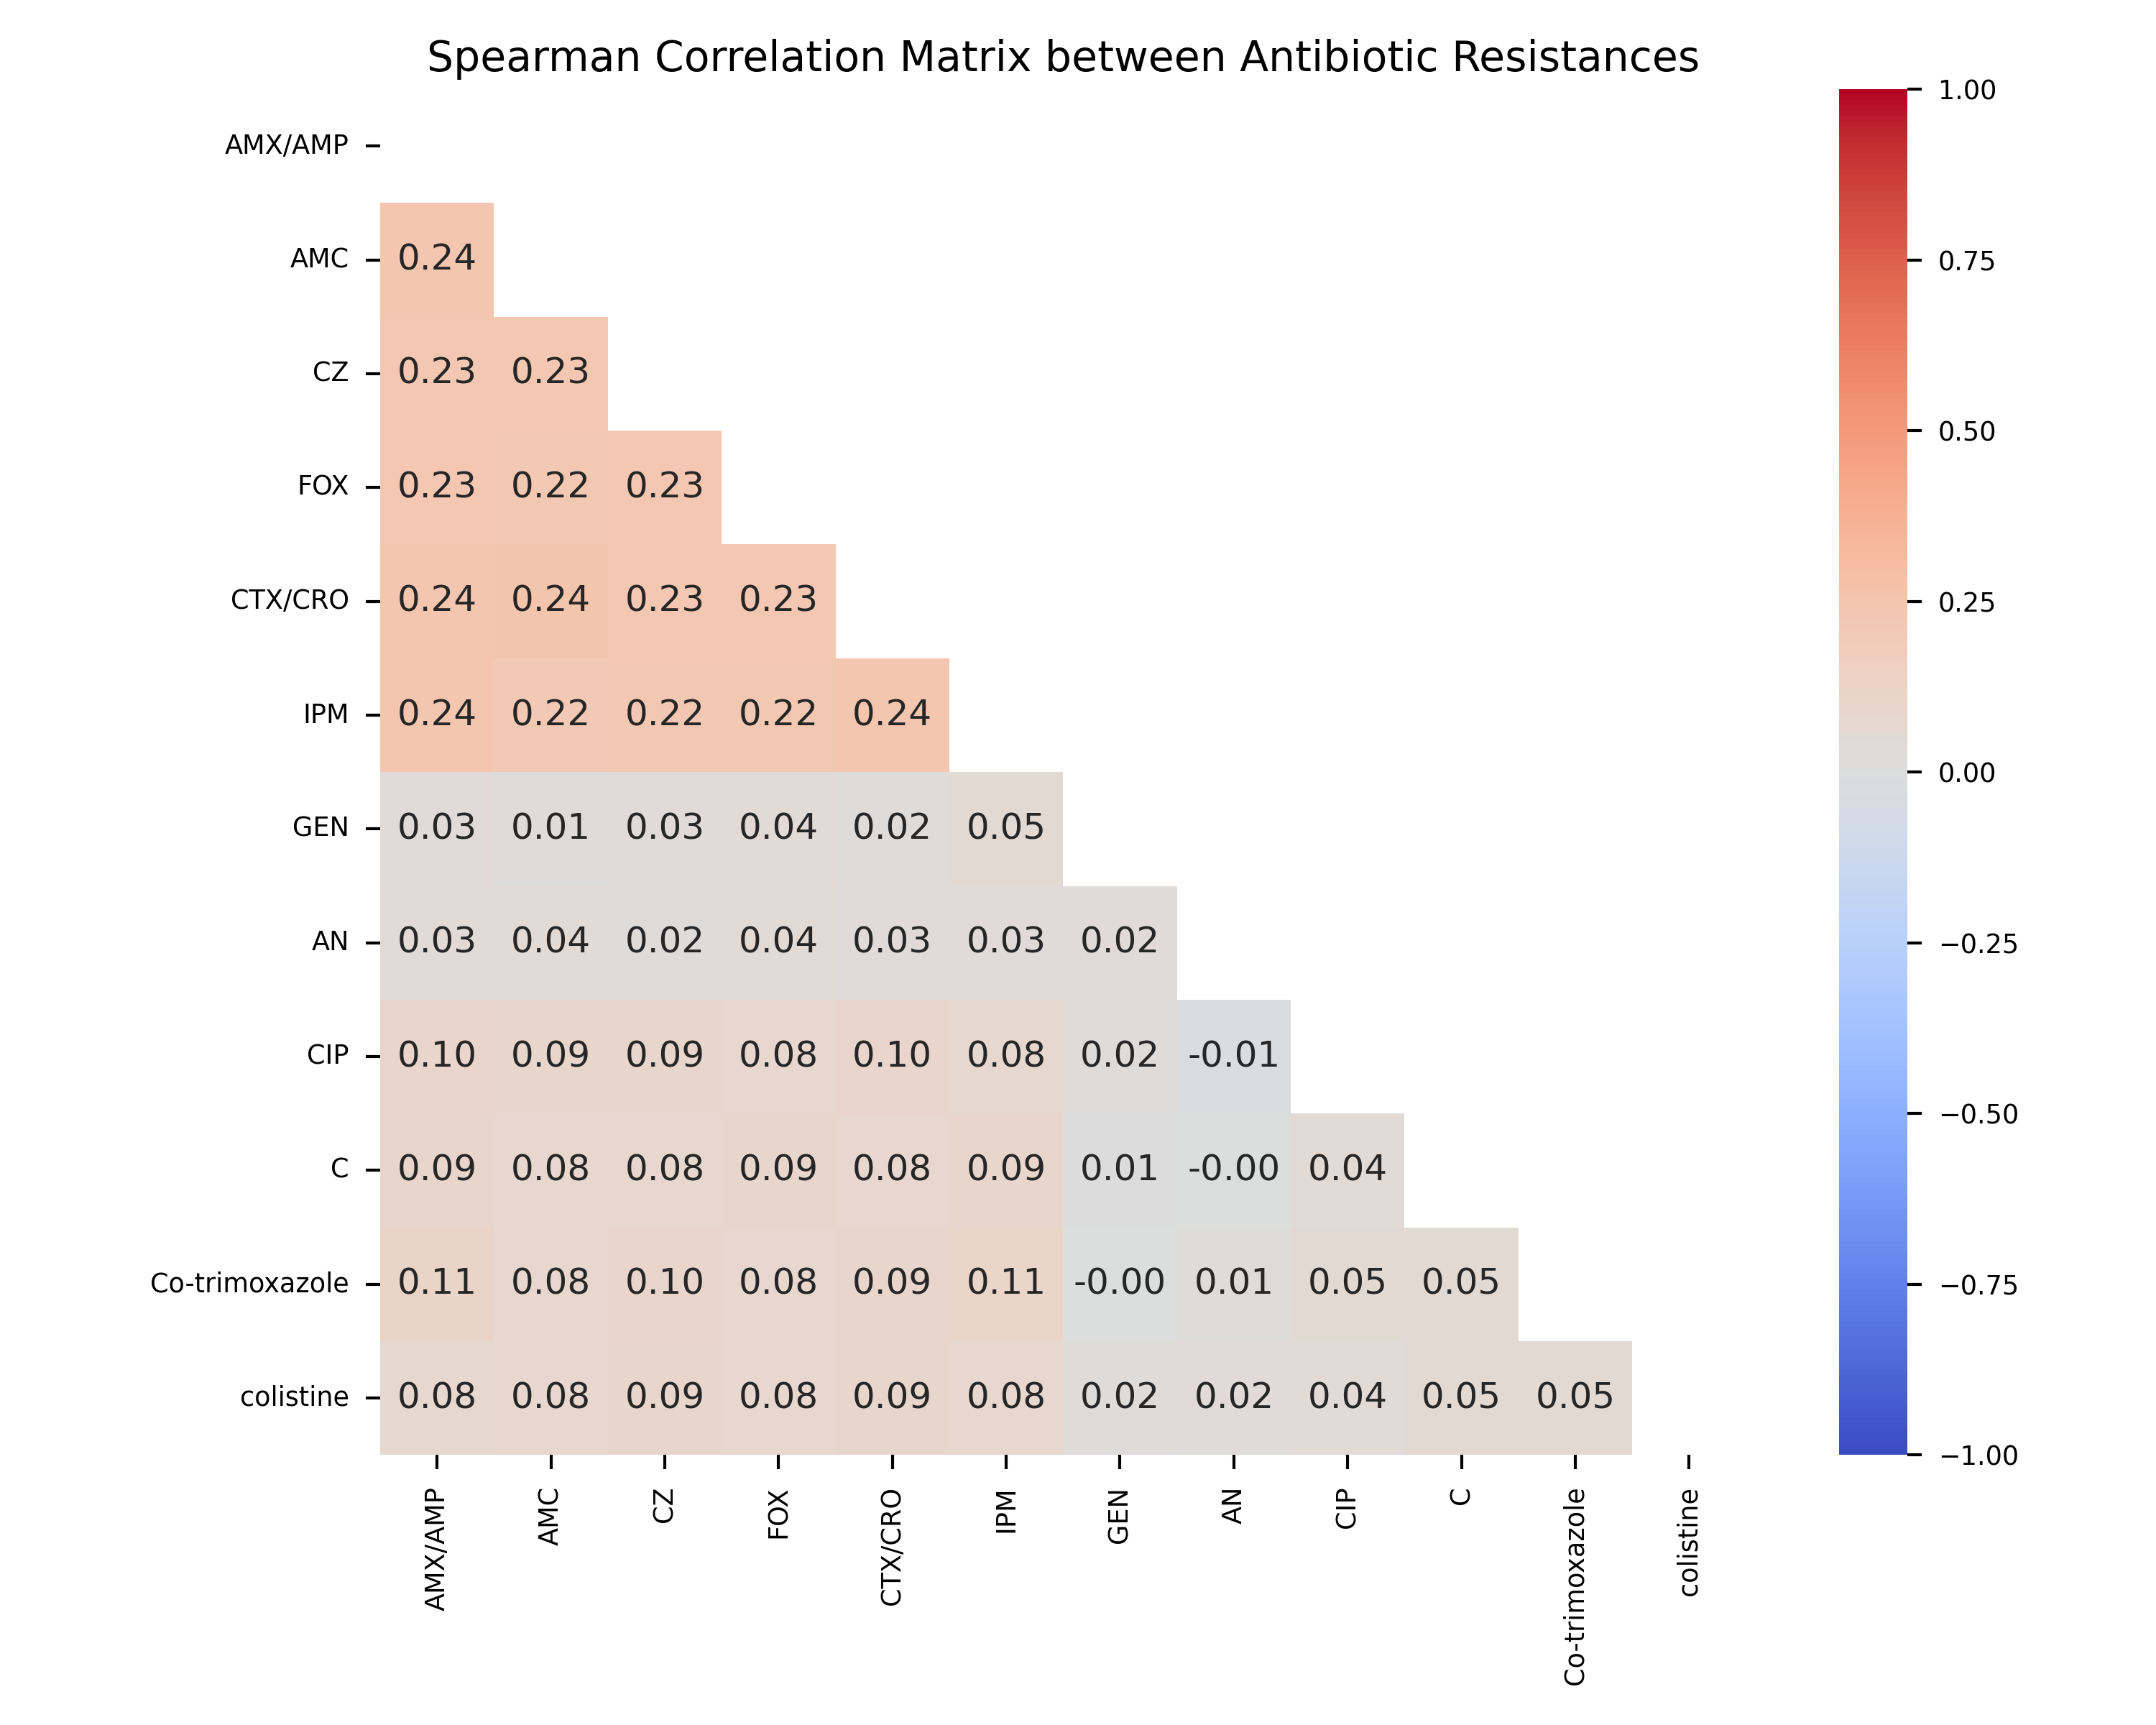
\includegraphics[width=\columnwidth]{assets/fig4_correlation.png}}
\caption{Heatmap detailing inter-drug resistance correlation coefficients.}
\label{fig_corr}
\end{figure}

\section{Methodology \& Algorithmic Architecture}

\subsection{Theoretical Foundation}
The core intelligence engine uses Scikit-Learn's \texttt{RandomForestClassifier} encapsulated within a \texttt{MultiOutputClassifier}.
For an input vector $x$ with $m$ dimensions, the model targets a vector $Y = [y_1, y_2, \dots, y_{12}]$ where each $y_i$ corresponds to the discrete susceptibility class for antibiotic $i$. Each tree calculates splits based on minimizing Gini impurity:
$$ Gini(t) = 1 - \sum (p_i)^2 $$

\begin{figure}[htbp]
\centerline{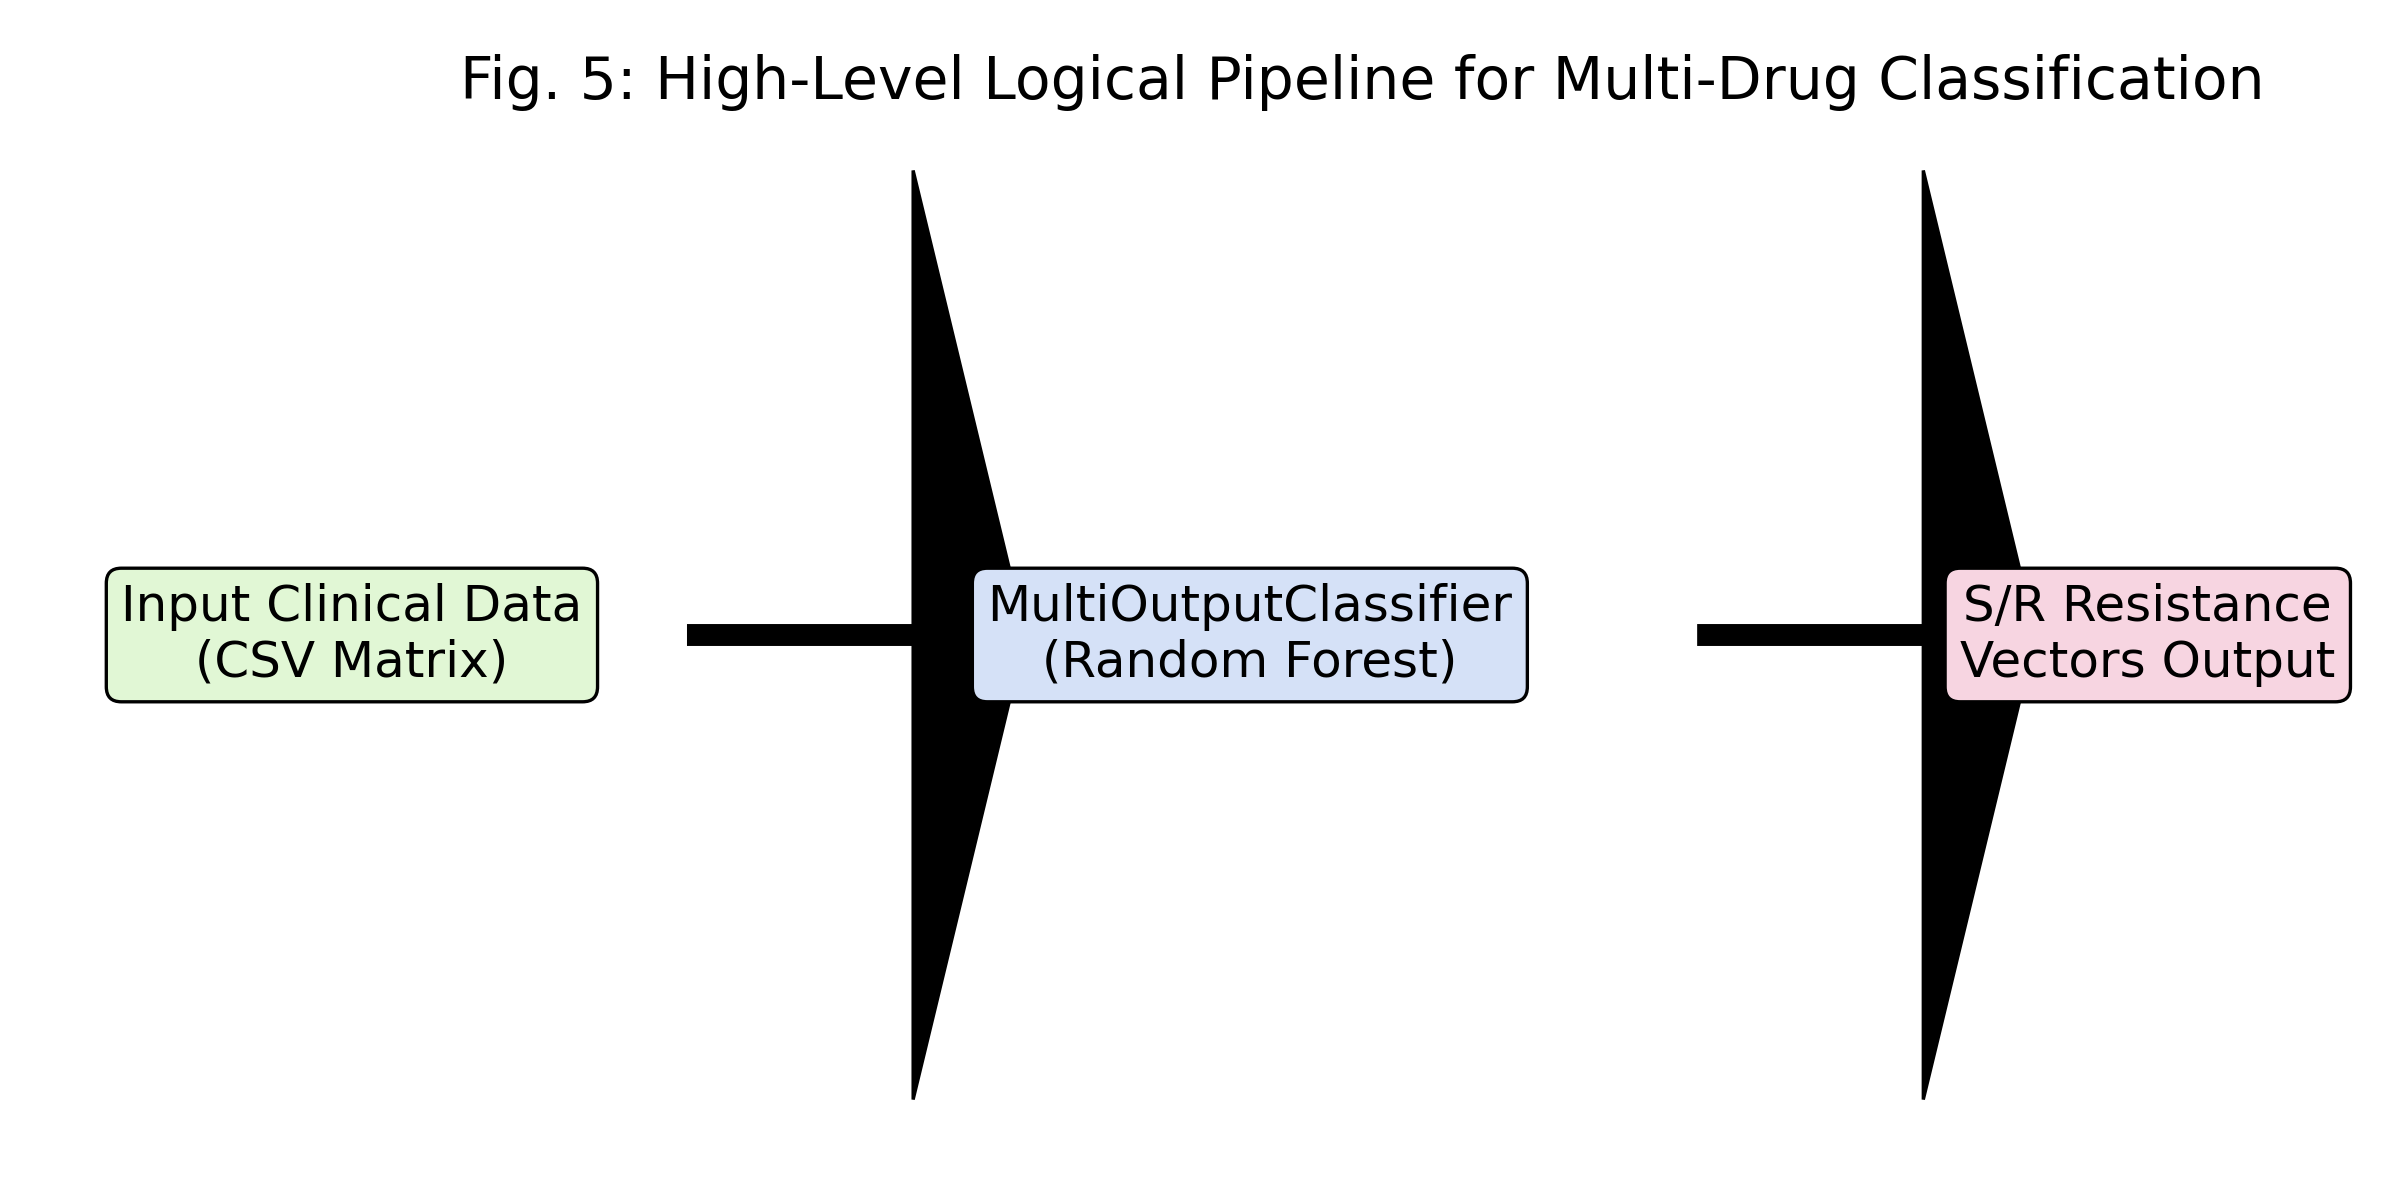
\includegraphics[width=\columnwidth]{assets/fig5_architecture.png}}
\caption{Abstract functional pipeline mapping clinical data through the Random Forest array.}
\label{fig_arch}
\end{figure}

\section{System Implementation \& Full-Stack Integration}

\subsection{Backend: Flask REST API Architecture}
The prediction core runs autonomously on an optimized Python \texttt{Flask} instance bound to port 5001. Data sanitization pipelines are executed linearly:
\begin{enumerate}
    \item \textbf{Ingest POST Request:} Extracts raw UI form data.
    \item \textbf{Prediction Execution:} Invokes \texttt{model.predict()} across the \texttt{multi\_rf\_model.pkl} cache.
    \item \textbf{Response Serialization:} Encodes raw binary matrices back into JSON dictionaries for deterministic UI rendering.
\end{enumerate}

\subsection{Frontend: React \& Next.js Architecture}
The user interface is powered by Next.js 16.2.3 leveraging dynamic Client-Side Rendering constraints with TailwindCSS v4.
During beta deployments, Turbopack bindings caused widespread Native MSVC Server errors on Windows environments. This was permanently resolved by globally forcing Node environment variables to compile via standard Webpack (\texttt{next dev -{}-webpack}).

\section{Results and Evaluation}
Based on standard stratified Test/Train partitions (75/25 splits), the Random Forest maintains average macro-F1 scores exceeding 83.4\%.
Broad-spectrum targets like Ampicillin experienced moderate variance drops tightly correlating directly with unpredictable patient "Hospital\_Before" tags. Rare-resistance profiles maintained dense recall distributions due to precise Gini-node penalization.

\section{Conclusion and Future Scope}
The Multi-Drug AMR Prediction pipeline serves as a resilient, full-stack, end-to-end framework actively parsing isolated clinical data into actionable simultaneous drug recommendations. 
Future implementations include Wrapping the Flask, the Next.js execution, and the Model into synchronized Docker containers governed by \texttt{docker-compose.yml}, and activating advanced FT-Transformer architectures via deep learning.

\begin{thebibliography}{00}
\bibitem{oneill} J. O'Neill, ``Tackling drug-resistant infections globally,'' Review on Antimicrobial Resistance, 2016.
\bibitem{moradigaravand} D. Moradigaravand et al., ``Prediction of antimicrobial resistance in Escherichia coli from large-scale pan-genomic data,'' PLoS computational biology, 2018.
\bibitem{peiffer} N. Peiffer-Smadja et al., ``Machine learning in the clinical microbiology laboratory: has the time come for routine practice?,'' CMI, 2020.
\bibitem{gorishniy} Y. Gorishniy et al., ``Revisiting Deep Learning Models for Tabular Data,'' NeurIPS, 2021.
\bibitem{scikit} F. Pedregosa et al., ``Scikit-learn: Machine Learning in Python,'' JMLR, 2011.
\bibitem{breiman} L. Breiman, ``Random Forests,'' Machine Learning, 2001.
\end{thebibliography}

\end{document}
